\documentclass[11pt, openany]{article}

\usepackage[T1]{fontenc}
\usepackage[utf8]{inputenc}
\usepackage[english, italian]{babel}
\usepackage{cancel}

\usepackage{hyperref}
\hypersetup{colorlinks=true,
	linkcolor=black,
	citecolor= black,
	filecolor=magenta,
	urlcolor=cyan,
}

\usepackage{geometry}
\geometry{
	a4paper,
	top=2.5cm,
	bottom=2cm,
	left=1.5cm,
	right=1.5cm,
	heightrounded,
	bindingoffset=5mm
}

\usepackage{amsmath}
\usepackage{amssymb}
\usepackage{amsthm}
\usepackage{tabularx}
\usepackage{booktabs}
\usepackage{caption}
\captionsetup{font = smaller}
\usepackage{enumitem}
\usepackage{blindtext}
\usepackage[x11names]{xcolor}
\usepackage{tcolorbox}
\usepackage{graphicx}
\usepackage{pdfpages}
\usepackage[export]{adjustbox}
\usepackage{cleveref}
\usepackage{multirow}
\usepackage{lipsum}



\theoremstyle{definition}
\newtheorem*{defn}{Definizione}
\newtheorem{exe}{Esercizio}[section]
\newtheorem{esem}{Esempio}[section]
\theoremstyle{plain}
\theoremstyle{remark}
\newtheorem*{warn}{ATTENZIONE}
\newtheorem*{svol}{Svolgimento}

\setcounter{secnumdepth}{-1}
\setcounter{tocdepth}{4}


\setlist[itemize]{nosep}
\usepackage{helvet}
\renewcommand{\familydefault}{\sfdefault}


\title{Relazione \\\textbf {Progetto A.A. 2022/2023 \\ ADAS made trivial: rappresentazione \underline{ispirata} alle
		interazioni in un sistema di guida autonoma}}
\author{Diciotti \hfill Matteo \\\\ 7072181 \and Manucci \hfill Agostino \\\\ 7084379 \and Montes Anacona \\ Àlvaro \\ 7117731}
\date{1 giugno 2023 - \today}

\begin{document}
	\maketitle
	\hrule
	\vspace{1cm}

	\part[Presentazione]{}
		\paragraph{Titolo}
			Progetto A.A. 2022/2023 – ADAS made trivial: rappresentazione \underline{ispirata} alle interazioni in un sistema di guida autonoma
		\paragraph{Autori}
			\footnotesize Lista degli autori ordinata per numero di matricola\\
			\normalsize
			\begin{tabularx}{\textwidth}[t]{p{4.5cm} p{3.5cm} p{2.5cm} r}
				\textbf{Matricola} 	& 	\textbf{Cognome} 	& 	\textbf{Nome} 	& \textbf{e-mail} 					\\\toprule
				7072181				&	Diciotti			&	Matteo			&	matteo.diciotti@stud.unifi.it	\\
				7084379				&	Mannucci			&	Agostino		&	agostino.mannucci@stud.unifi.it	\\
				7117731				&	Montes Anacona		&	Álvaro			&	alvaro.montes@stud.unifi.it
			\end{tabularx}

		\paragraph{Obbiettivo}
			Obiettivo del progetto è costruire un’architettura, estremamente stilizzata e rivisitata, per sistemi ADAS, descrivendo possibili interazioni e alcuni comportamenti tra componenti in scenari specifici.

	\part{Introduzione}
		\paragraph{Introduzione al progetto}
			Un \textit{\textbf{A}dvanced \textbf{D}river \textbf{A}ssistance \textbf{S}ystem} è un sistema composto da varie componenti che cooperano affinché un veicolo o un mezzo possano assistere un conducente nella guida e in alcuni contesti sostituirsi al guidatore stesso.\\
			Il progetto realizzato cerca di riprodurre fedelmente il sistema simulativo di un ADAS presentato nella richiesta\footnote{Per visionare la richiesta dell'elaborato riferirsi al documento Allegato\_1.pdf compreso nella cartella del progetto} dell'elaborato nella quale sono definite varie componenti suddivise in quattro gruppi: \textit{interfaccia}, \textit{attuatori}, \textit{sensori} e \textit{controllo}.\\
			La simulazione è resa effettiva dall'inserimento di stringhe rappresentanti le azioni che dovrebbero essere eseguite dalle varie componenti di un ADAS in dei file di log specifici per ogni componente. In particolare le componenti implementate sono nove, sette obbligatorie e due facoltative\footnote{Per conoscere quali elementi facoltativi sono stati implementati visionare la tabella~\ref{tab:facoltativi}}.\\
			I \textit{sensori}, attraverso l'acquisizione di dati da file predefiniti o da sorgenti casuali, simulano l'acquisizione di dati da parte di sensori reali e li inviano all'unica componente di controllo, la componente \textit{Central ECU}. Gli \textit{attuatori} ricevono messaggi dall'unità di controllo ed eseguono scritture nell'apposito file di log per simulare la messa in atto dell'attuazione del comando su di un attuatore reale. Infine la componente con cui si interfaccia l'esecutore del programma è la \textit{Human-Machine Interface} che simula l'interfaccia del guidatore attendendo comandi (in questo caso scritti su di un terminale) e mostrando i risultati e le conseguenze dei propri comandi (nel caso della simulazione saranno scritti su di un differente terminale tutti i comandi che l'unita di controllo centrale ha inviato alle varie componenti).

		\paragraph{Impostazione del lavoro}
			Al fine di realizzare un sistema che simulasse un ADAS sono state eseguite alcune fasi per il completamento del programma: l'analisi delle richieste, la strutturazione teorica dell'architettura del sistema, l'implementazione pratica, la verifica e revisione dell'elaborato.\\
			Ad una prima fase di studio delle richieste congiunta tra gli autori del progetto è immediatamente succeduta la fase di strutturazione dello stesso, anch'essa svolta unitamente tra i relatori, giungendo alla teorizzazione dell'architettura mostrata in figura~\ref{fig:gerarchia}. Sono stati quindi divisi i lavori per l'implementazione del programma tra i componenti del gruppo e uniti gli elaborati in un unico componimento comprensivo di makefile e file binari per l'esecuzione in modalità \textit{ARTIFICIALE} del programma. Sono state quindi eseguite ciclicamente le due fasi di verifica e di revisione: nella prima fase sono stati svolti test per verificare il corretto funzionamento dell'elaborato per entrambe le modalità e nella seconda fase sono state apportate le modifiche necessarie affinché il programma producesse i risultati attesi. Infine e` stata prodotta la presente relazione.
	\part{Specifiche}
		\paragraph{Caratteristiche HW e SW}
		Per l'implementazione sono stati utilizzati tre hardware differenti con tre sistemi operativi differenti:
		\begin{itemize}
			\item \textbf{ArchLinux}, architettura x86\_64, kernel Linux 6.1.34-1-LTS
			\item \textbf{Manjaro 23.0.0}, architettura x86\_64, kernel Linux 5.15.114-2-MANJARO
			\item \textbf{Ubuntu 20.04}, architettura x86\_64, kernel Linux 5.15.0-75-generic
		\end{itemize}
		Il progetto è stato ideato avendo come obbiettivo un programma portatile che fosse preimpostato per eseguire su di un sistema \textbf{\underline{Ubuntu Linux 22.04}}.
		\paragraph{Istruzioni compilazione ed esecuzione}
			Nel presente paragrafo si mostrano i passaggi necessari affinche si possa eseguire il programma sul proprio dispositivo:
			\subparagraph{Estrazione e compilazione}
				\begin{enumerate}
					\item Estrarre il file .zip in una cartella a piacimento. (Esempi comando: \texttt{tar~-x~\$PROJECT\_NAME\$; \texttt{7z~x~\$PROJECT\_NAME\$}});
					\item Spostarsi nella cartella creatasi con l'estrazione. (Esempio comando: \texttt{cd~./\$PROJECT\_NAME\_FOLDER\$});
					\item Eseguire il comando di installazione e la compilazione del programma \texttt{make install}.
				\end{enumerate}
				Terminata questa procedura il programma dovrebbe risultare pronto per l'esecuzione.
				\subparagraph{Esecuzione}
					\begin{enumerate}
						\item Assicurarsi di essere con un terminale nella directory sorgente del programma, la stessa contenente le cartelle bin, src, include etc. e il file eseguibile ADAS-simulator.
						\item Avviare l'inizializzazione e l'esecuzione del programma tramite la chiamata di \texttt{./ADAS-simulator \$MODALITÀ\$}, dove \texttt{\$MODALITÀ\$} rappresenta la modalità \texttt{ARTIFICIALE} o \texttt{NORMALE} del programma\footnote{Per la comprensione delle differenze delle modalita di esecuzione riferirsi al paragrafo 4 della richiesta \textit{Allegato\_01.pdf}}. Oltre al secondo argomento (il quale risulta obbligatorio, pena la mancata esecuzione del programma e la restituzione di un errore), il comando supporta anche l'opzione \texttt{$--$term} nella quale si può specificare l'emulatore di terminale che si desidera visualizzare come terminale di output. L'emulatore impostato di default è gnome-teminal.
						\item Eseguito il comando dovrebbe aprirsi automaticamente un nuovo terminale rappresentante il terminale di output. Non eseguire alcun comando sul terminale di output e posizionarsi sul terminale di input, ovvero il terminale nel quale è stato eseguito il comando di avvio del programma.
						\item Il programma è inizializzato, si possono quindi eseguire i comandi INIZIO, PARCHEGGIO per iniziare l'esecuzione del programma e successivamente ARRESTO per simulare un arresto del veicolo\footnote{Per la comprensione dei comandi inseribili dal terminale rifarsi al paragrafo 2, sotto-paragrafo \textit{Human-Machine Interface}, della richiesta \textit{Allegato\_01.pdf}}.
				\end{enumerate}

				\begin{figure}[b!]
					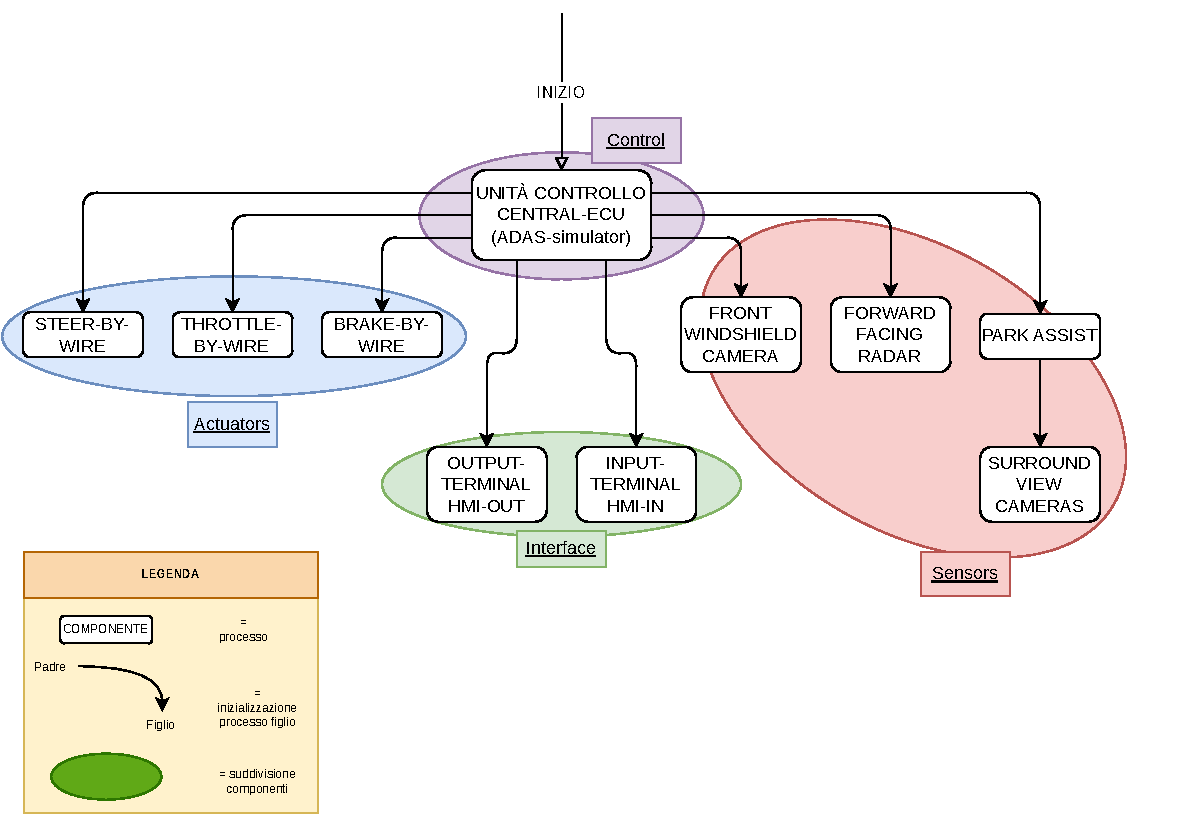
\includegraphics[scale=0.8, center]{./include/SO_Progetto_Diagrammi-Gerarchia.pdf}
					\caption{In figura è mostrata la gerarchia implementata nel programma, nel quale la \textit{central-ECU} rappresenta il processo antenato di tutte gli altri processi.}
					\label{fig:gerarchia}
				\end{figure}

		\paragraph{Elementi facoltativi}
			La tabella a pagina~\pageref{tab:facoltativi} mostra gli elementi facoltativi implementati seguiti da una breve descrizione dell'implementazione.
			\begin{tcolorbox}[width=\textwidth,colback={Cornsilk2}]
				\begin{tabularx}{\textwidth}{lXcX}
					\textbf{\#}	&	\textbf{Elemento facoltativo}	&	\textbf{Realizzato (SI/NO)}	&	\textbf{Descrizione dell'implementazione con indicazione del metodo/i principale/i} \\\toprule\vspace{.1cm}
					1	&	Ad ogni accelerazione, c’è una probabilità di $10^{-5}$ che l’acceleratore fallisca. In tal caso, il componente \textit{throttle control} invia un \underline{segnale} alla \textit{central ECU} per evidenziare tale evento, e la Central ECU avvia la procedura di \textit{ARRESTO} & SI	&	Metodo: throttle-control $\rightarrow$ throttle\_failed(). Il metodo, tramite la funzione \texttt{rand()} della \texttt{libc} ottiene un numero aleatorio il cui modulo per 10000 simula una probabilita del 1 su $10^5$ se eguagliato a 0\footnote{La probabilita non risulta esattamente $10^-5$ dato l'intervallo di valori producibili da \texttt{rand()}, ma la differenza dovrebbe essere trascurabile ai fini del progetto.} \\\vspace{0.1cm}
					2	&	Componente \textit{forward facing radar}	&	SI	&	Sorgente \textit{bytes-sensors.c}. Il processo esegue un ciclo infinito di letture, invii e scritture su file di log.\\\vspace{0.1cm}
					3	&	Quando si attiva l’interazione con park assist, la \textit{Central ECU} sospende (o rimuove) tutti i sensori e attuatori, tranne \textit{park assist} e \textit{surround view cameras}	&	SI	&	Metodo: \textit{central-ECU }$\rightarrow$ \dots. La metodo invia un segnale di terminazione immediata a tutti gli attuatori e ai sensori diversi da quelli specificati.\\\vspace{0.1cm}
					4	&	Il componente \textit{park assist} non è generato all'avvio del sistema, ma creato dalla \textit{Central ECU} al bisogno	&	\multirow{4}*{SI}	&	La \textit{central-ECU} esegue la \texttt{fork} per la creazione di \textit{park-assist} in \dots	\\\vspace{0.1cm}
					5	&	Se il componente \textit{surround view cameras} è implementato, \textit{park assist} trasmette a \textit{Central ECU} anche i byte ricevuti da \textit{surround view cameras}	&	SI	&	Nel ciclo principale di \textit{park-assit} si esegue una \texttt{read} da \textit{surround-view} e una \texttt{write} dei dati ricevuti sul pipe \textit{assist.pipe} \\\vspace{0.1cm}
					6	&	Componente \textit{surround view cameras}	&	SI	&	Sorgente \textit{bytes-sensors.c}. Vedi facoltativo 2 - \textit{forward facing radar}	\\\vspace{0.1cm}
					7	&	Il comando di \textit{PARCHEGGIO} potrebbe arrivare mentre i vari attuatori stanno eseguendo ulteriori comandi (accelerare o sterzare). I vari attuatori interrompono le loro azioni, per avviare le procedure di parcheggio	&	SI	&	Nella \textit{central-ECU}, metodo \dots, si esegue segnalazione di interruzione immediata che interrompe immediatamente i processi.\\
					8	&	Se la \textit{Central ECU }riceve il segnale di fallimento accelerazione da \textit{throttle control}, imposta la velocità a 0 e invia all'output della \textit{HMI} un messaggio di totale terminazione dell'esecuzione	&	SI	&	Nella \textit{central-ECU}, una volta ricevuto il segnale di \textit{PERICOLO} si esegue la procedura di arresto e si termina l'esecuzione \dots
				\end{tabularx}
				\label{tab:facoltativi}
			\end{tcolorbox}

	\part{Descrizione architettura sistema}
		Nella seguente sezione viene presentata l'architettura del progetto e le scelte implementative prese, cercando di descrivere i motivi che hanno portato alle singole decisioni prese.

		\paragraph{Implementazione componenti}
			\footnotesize Segue una tabella nella quale si mostrano quali sorgenti implementano le componenti
			\normalsize

			\begin{tcolorbox}[width=\textwidth,colback={Cornsilk2}]\label{tab:sorgenti}
				\begin{tabularx}{\textwidth}{p{8cm}  l}
					\textbf{Componente}			&	\textbf{Sorgente}	\\\toprule
					Human-Machine Interface 	& 	hmi-input.c			\\
												&	hmi-output.c		\\\midrule
					steer-by-wire				&	steer-by-wire.c		\\\midrule
					throttle control			&	throttle-control.c	\\\midrule
					brake-by-wire				&	brake-by-wire		\\\midrule
					front windshield camera		&	windshield-camera.c	\\\midrule
					forward facing radar		&	bytes-sensors.c		\\\midrule
					park assist					&	park-assist.c		\\\midrule
					surround view cameras		&	bytes.sensors.c		\\\midrule
					central ECU					&	central-ECU.c


				\end{tabularx}
			\end{tcolorbox}

		\paragraph{Gerarchia del programma}
			La gerarchia del progetto è stata ottenuta dalla richiesta cercando di massimizzare la semplicità.\\
			Questa rappresenta lo scheletro del progetto e definisce quindi il flusso di lavoro dello stesso. In particolare si può notare in figura~\ref{fig:gerarchia} che esistono due soli processi che inizializzano dei figli, ovvero l'unita di controllo centrale \textit{central-ECU}, che rappresenta anche il programma genitore di tutto il sistema, e \textit{park-assist}, che inizializza il suo unico figlio \textit{surround-view cameras}.\\
			È stato scelto di rendere l'unità di controllo genitore di tutto il sistema dato essere in collegamento con la quasi totalità dei processi agenti, cosicché il sistema fosse interamente inizializzato in un solo intervallo temporale da un unico processo.\\
			Infatti nella \textit{central-ECU} vengono immediatamente inizializzati i pipe, dopodiché vengono eseguite varie \texttt{fork} per la creazione e la connessione in lettura/scrittura ai pipe degli attuatori, delle due componenti relative alla \textit{Human-Machine Interface} ed infine i due sensori \textit{front windshield camera} e \textit{forward facing radar}. L'unico componente figlio della \textit{central-ECU} non immediatamente inizializzato rimane \textit{park-assist}\footnote{La decisione di non inizializzare il componente immediatamente deriva dalla richiesta, ovvero dall'elemento facoltativo numero 4. Vedi la tabella di pagina~\pageref{tab:facoltativi}.} il quale verrà messo in esecuzione dalla stessa unità di controllo quando questa riceverà un comando di \textit{PARCHEGGIO} dall'interfaccia oppure dal sensore \textit{windshield}.\\
			Per limitare il tempo di inizializzazione della componente \textit{park assist}, che a sua volta deve inizializzare il figlio \textit{suround-view cameras} al proprio avvio e che quindi richiede qualche istante di tempo, e per poter mantenere semplice la struttura del sistema è stato deciso di rendere la \textit{central-ECU} "server" nella connessione socket tra questa e \textit{park assist}. In questo modo l'unità di controllo inizializzerà il server/socket \texttt{assist.sock} al momento dell'inizializzazione del sistema, non rendendo però necessario avviare la componente \textit{park assist} fintantoché non ve ne sarà bisogno. Quando questa verrà avviata dovrà solo mettersi in connessione con la socket già creata precedentemente, risparmiando il tempo di inizializzazione della stessa.\footnote{Sebbene possa sembrare contro-intuitivo che la componente \textit{park assist} rappresenti il client della connessione clinet/server (dato che sembrerebbe essere proprio \textit{park assist} a svolgere un servizio per l'unità di controllo) risulta molto conveniente rendere la \textit{central-ECU} il server poiché, essendo il canale comunicativo esclusivo per i due processi, non modifica il comportamento del sistema e rende l'inizializzazione del figlio più rapida.}\\
			All'avvio della procedura di parcheggio, quindi, la \textit{central-ECU} avvierà la componente \textit{park-assist}, la quale si connetterà alla socket e inizializzerà \textit{surround-view-cameras}. Le due componenti leggeranno per i 30 secondi successivi dati da sorgenti binarie e se in queste non risulteranno particolari pattern\footnote{Per conoscere i pattern binari (espressi in codifica esadecimale) prendere visione del paragrafo 2, sotto-paragrafo \textit{Componente central-ECU} della richiesta \textit{Allegato\_01.pdf}} allora l'esecuzione del parcheggio risulterà conclusa e il processo terminerà con successo, in caso invece almeno uno dei pattern succitati dovesse essere presente nei dati acquisiti dalle componenti allora la procedura di parcheggio terminerà immediatamente, ovvero non appena le uguaglianze vengono evidenziate, e si riavvierà immediatamente la procedura di parcheggio.

		\paragraph{IPC nel sistema}
			In figura~\ref{fig:comunicazione}, a pagina~\pageref{fig:comunicazione}, si mostra una schematizzazione molto stilizzata della rete comunicativa del sistema.
			Il metodo di comunicazione maggiormente sfruttato all'interno del sistema è indubbiamente il \textbf{pipe} il quale struttura 8 canali di comunicazione su 9 (segnali esclusi). Il motivo della scelta dei \textbf{pipe} a discapito di altri metodi risiede nel fatto che le comunicazioni sono sostanzialmente unidirezionali (sensori $\rightarrow$ unità di controllo, unità di controllo $\rightarrow$ attuatori, con due evidenti eccezioni di \textit{park assist} e di \textit{surround-view-cameras}). La scelta ha permesso di implementare un sistema relativamente semplice, con un'unica \textbf{socket}, struttura più complessa da implementare e gestire.\\
			Il protocollo di gestione dei canali risulta unico per tutte le tipologie di canali e per tutti i processi: il processo padre, l'unico processo che comunica con i propri processi figli, produce ed inizializza correttamente il file \texttt{.pipe} o \texttt{.sock} (rappresentante socket \texttt{UNIX}) nella directory \textit{tmp} (dopo aver avuto l'accortezza di eliminare creazioni pendenti da vecchie esecuzioni tramite un \texttt{unlink}), il processo figlio si connette con  l'adeguata procedura, differente tra pipe e socket, al canale di comunicazione nella fase inizializzazione del processo. Se la connessione non dovesse riuscire (se la \texttt{open} o la \texttt{connect} dovessero terminare con un errore) il figlio terminerebbe con codice di errore \texttt{EXIT\_FAILURE} e stamperebbe lo stack dell'errore nello \textit{stderr}.\\
			Per l'implementazione del parcheggio il canale di comunicazione assume sembianze di una socket per evitare di dover terminare il programma \textit{park-assist} ogni volta che la \textit{central-ECU} riceve da questo uno dei pattern non ammissibili, che simulano una situazione di parcheggio non accettabile. Il protocollo prevede che ad ogni ciclo \textit{park assist} riceva da \textit{surround-view cameras} i byte da inviare alla \textit{central-ECU} e che li invii, assieme da quelli letti dalla sorgente binaria. Se, eseguito l'invio, riceve dalla \textit{central-ECU} un messaggio che indica la necessit di riavvio, allora \dots
			\begin{figure}[t]
				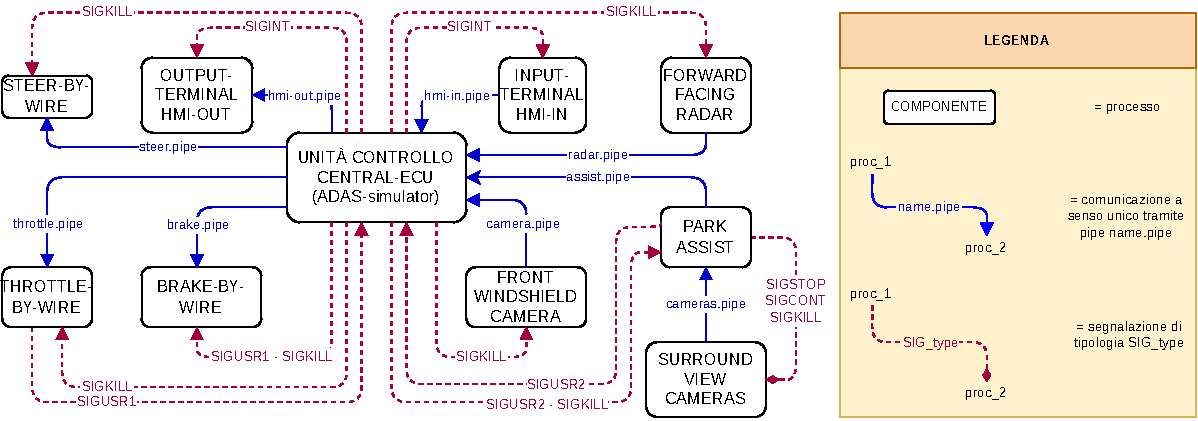
\includegraphics[scale=0.9, center]{./include/SO_Progetto_Diagrammi-Comunicazione.pdf}
				\caption{In figura sono rappresentati tutti e soli i percorsi comunicativi inseriti nel sistema: sono presenti 9 pipe e 15 percorsi di segnalazioni inviate dai processi del sistema ad altri processi dello stesso.}
				\label{fig:comunicazione}
			\end{figure}
		\paragraph{Gestione dei log}
			\lipsum







			\newpage


	\newpage
	\hrule
	\tableofcontents

\end{document}